\documentclass{article}
\usepackage[utf8]{inputenc}
\usepackage{a4wide}
\usepackage{amsmath}
\usepackage{amssymb}
\usepackage{fancyhdr}
\usepackage{lastpage}
\usepackage{graphicx}
\usepackage[danish]{babel}
\usepackage{float}
\usepackage{appendix}
\usepackage{xcolor}
\usepackage{listings}
\usepackage{lipsum}  
\usepackage{fancyref}
%\usepackage{varioref}

\usepackage{svg}
\usepackage{caption}
\usepackage{subcaption}
\usepackage{mdframed}
\usepackage{placeins}
\usepackage{algpseudocode}
\usepackage{booktabs}
\usepackage{pdfpages}

\usepackage{hyperref}
\hypersetup{
    colorlinks,
    citecolor=black,
    filecolor=black,
    linkcolor=black,
    urlcolor=black
}

% bokse
\usepackage[framemethod=default]{mdframed}

% coding
\usepackage{pythonhighlight}

\newcommand{\code}{\texttt}

% sources
\usepackage[
backend=biber,
style=apa,
]{biblatex}
\addbibresource{sources.bib}

% Documentation for fancyref:
% https://mirrors.dotsrc.org/ctan/macros/latex/contrib/fancyref/fancyref.pdf

% Redefine commands for danish - add more when needed, see above pdf p. 8 - 10
\renewcommand*{\Frefeqname}{ligning}
\renewcommand*{\Frefsecname}{sektion}
\renewcommand*{\tablename}{tabel}

\renewcommand{\fancyrefdefaultformat}{plain}

%\renewcommand*{\pagename}{side}
%\renewcommand*{\Frefonname}{på}
%\renewcommand*{\Frefseename}{se}

% path for image
\graphicspath{ {./images/} }


\usepackage{eso-pic}
\newcommand\BackgroundPic{%
\put(0,0){%
\parbox[b][\paperheight]{\paperwidth}{%
\vfill
\centering
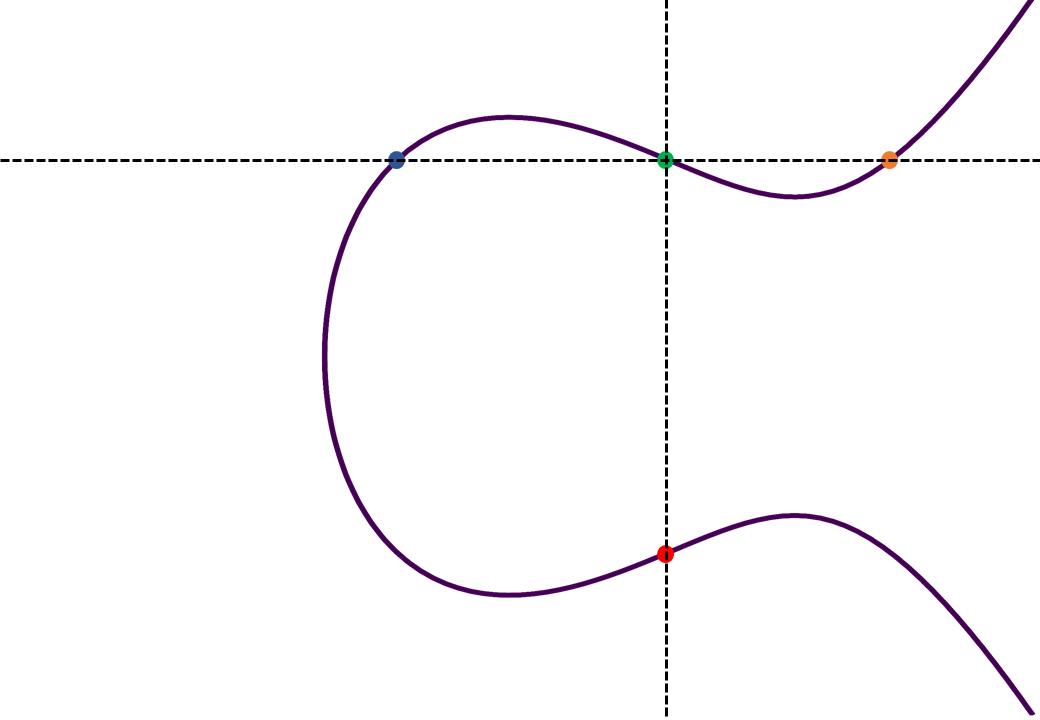
\includegraphics[angle=90, width=\paperwidth,height=\paperheight,%
keepaspectratio]{final.png}%
\vfill
}}}

\title{
    \vspace{7cm}
    \\
    Eliptisk kurvekryptografi
    \\
}
\author{Philip Rying}
\date{18-03-2022}

\pagestyle{fancy}
\fancyhf{}
\rhead{\leftmark}
\lhead{Philip Rying}
\rfoot{\thepage{} af \pageref{LastPage}}

\begin{document}
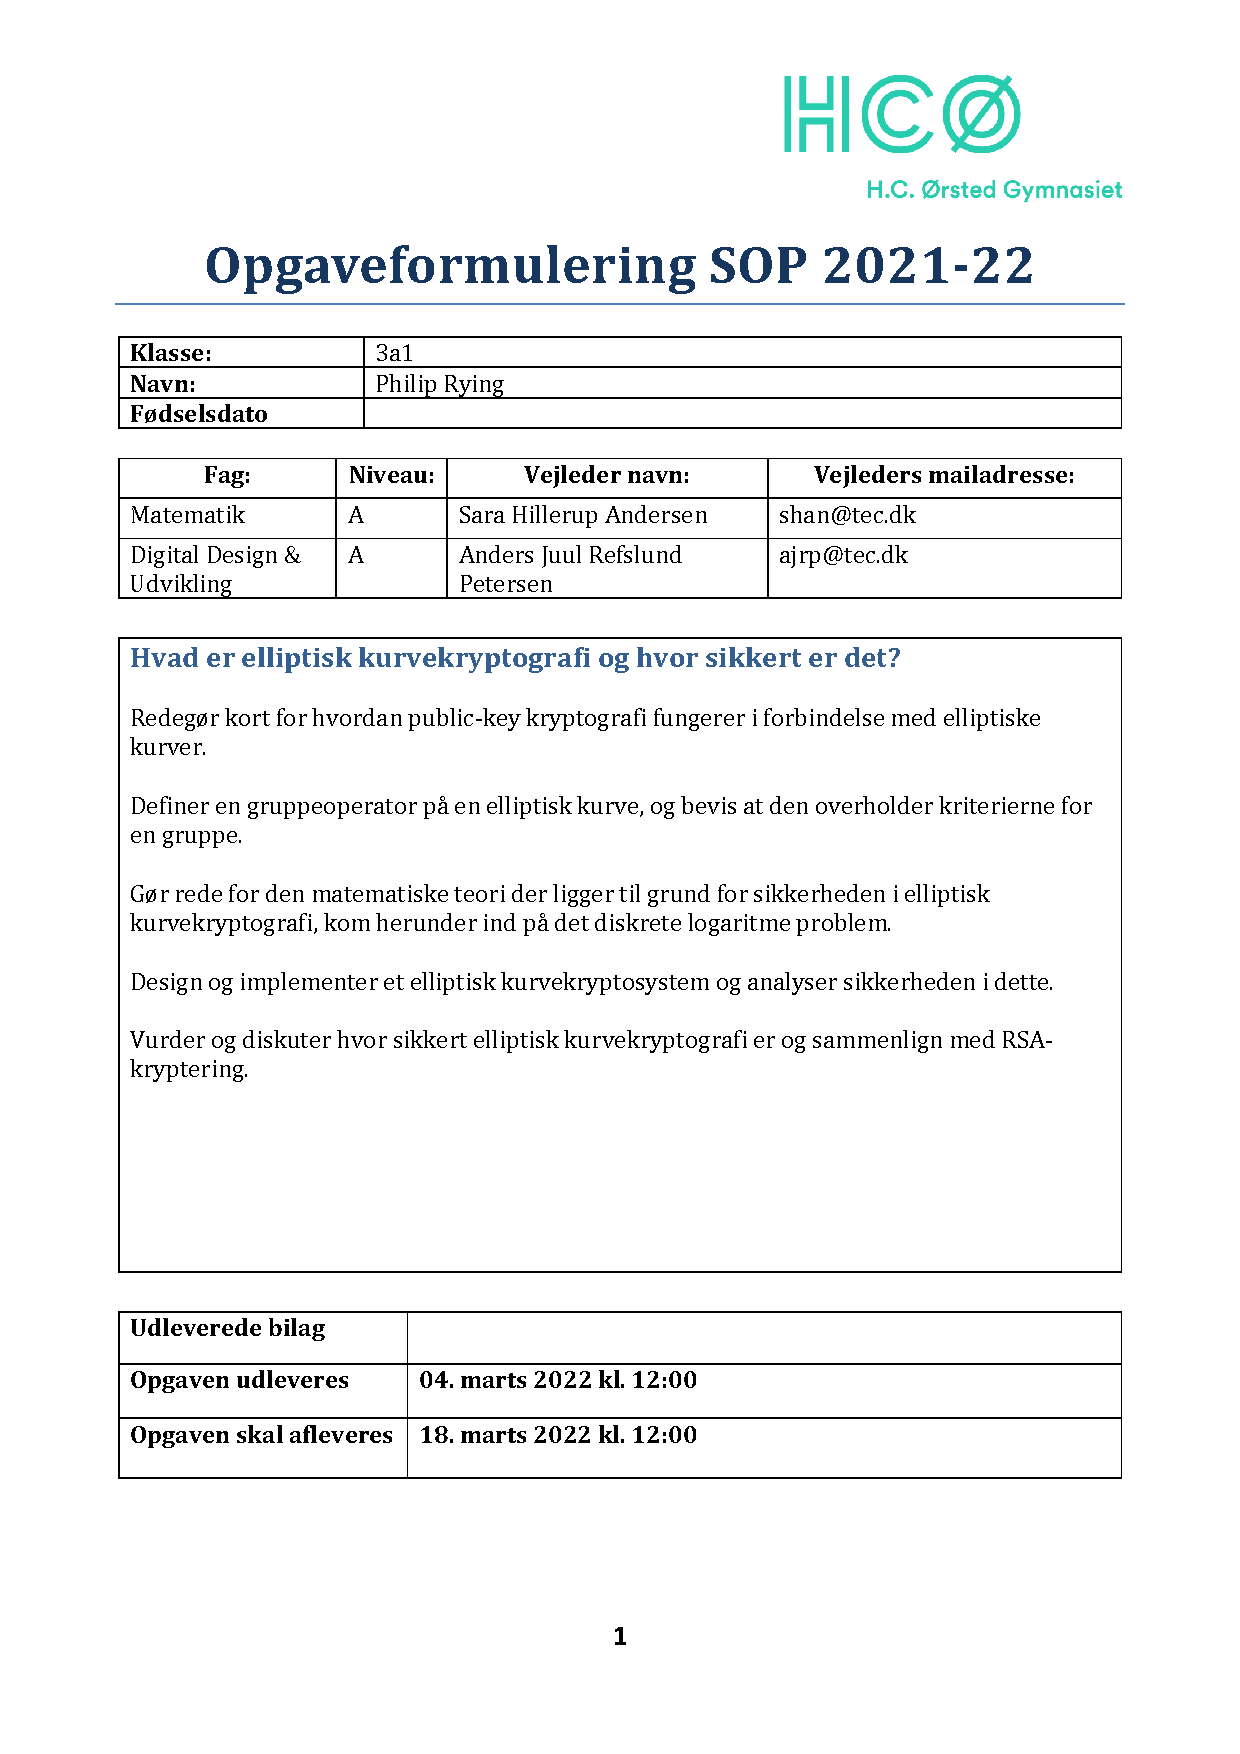
\includepdf[pages={1}]{Philip Rying 3a1 SOP Opgaveformulering.pdf}
\AddToShipoutPicture*{\BackgroundPic}
\maketitle
\newpage
\begin{abstract}
Følgende opgave undersøger sikkerheden ved elliptisk kurvekryptografi. 
Der redegøres for elliptiske kurver hvorefter gruppestrukturen på dem bliver præsenteret. Herefter gives der en udledning for additionen af punkter i gruppen hvorefter begrebet skalarmultiplikation introduceres. Her bliver tiden for at lave $n$ additioner reduceret til $O(log_{2}n)$ i stedet for $O(n)$. Dernæst bliver elliptiske kurver på endelige legemer defineret, så en computer kan regne på dem. Herefter kigges der på hvordan elliptiske kurver kan anvendes indenfor kryptografi, hvor begrebet \textit{assymetrisk kryptering} introduceres. Algoritmen for et \code{Elliptic Curve Diffie Hellmann key exchange} gennemgås hvor der redegøres for det diskrete logaritmeproblem. Egen data fra en simulation af offentlig nøgle-generering sammenlignes med privat-nøgle brydning. Det ses at krypteringstiden stiger lineært, mens tiden for at bryde krypteringen stiger eksponentielt for bitlængden af privatnøglen. Der designes et system til elliptisk kurvekryptografi, hvor der med pseudokode redegøres for addition på en elliptisk kurve samt skalarmultiplikation. Sikkerheden i det implementerede system bliver vurderet som sikkert så langt tid, at man kan stole på den anden part. Til sidst sammenlignes elliptisk kurvekryptosystemer med RSA, hvor det konkluderes at en meget kortere key-længde for Elliptisk kurve kryptografi er nødvendig for samme "sikkerhed" som i et RSA-kryptosystem.
\end{abstract}
\newpage

\tableofcontents

\newpage
\section{Indledning}

Op indtil 1970'erne var alt kryptering baseret på \textit{symmetriske-funktioner}. Dette betød, at hvis to parter skulle kunne kommunikere sikkert, var de nødt til at møde fysisk først og blive enige om en \textit{fælles hemmelighed}. Op indtil det 20. århundrede var symmetrisk kryptering tilfredsstillende, men på baggrund af anden verdenskrig og internettes fødsel steg motivationen for at lave et system, hvor man kunne kommunikere sikkert uden at kende hinanden på forhånd.
Denne type kryptografi er kendt som \textit{assymetrisk-} eller \textit{public-key} kryptering og går ud på, at man har en offentlig- og privat nøgle. Den grundlæggende idé er, at man bruger den offentlige nøgle til at \textit{kryptere} beskeder, mens den private nøgle bruges til at \textit{dekryptere} beskeden og holdes altså privat (\cite{seanriley2017}). For at lave et sådan system har man brug for et sæt af algoritmer, hvor det er nemt at gå den ene vej, men meget svært at gå den anden. Den første, og til dags dato, mest anvendte er RSA-kryptering. Dens sikkerhed bygger på, at det er nemt at gange to store primtal sammen, men at faktorisere produktet til dets to primtal er svært \textit{(Diskrete logaritmeproblem)}. Problemet ved RSA-kryptering er dog, at der i dag er fundet algoritmer, som kan løse det diskrete logaritmeproblem på smartere måder en rent gætværk.  Dette har gjort, at RSA-nøglers længde har været nødt til at blive længere og længere efterhånden som computere er blevet hurtigere. Et nyt system som bygger på elliptiske kurver, har dog potentiale til at overtage for RSA-kryptering, da det diskrete logaritmeproblem for elliptisk kurvekryptografi, viser sig sværere at løse. 
I følgende opgave undersøges elliptisk kurvekryptografi fra definitionen af en elliptisk kurve, helt til implementering af et elliptisk kurvekryptosystem. Til sidst vurderes sikkerheden af det implementerede system, hvorefter det sammenlignes med RSA. 
\newpage

\section{Elliptiske Kurver}\label{sec:elliptiske_kurver}
I følgende afsnit redegøres der for elliptiske kurver på Weierstrass' normalform. Først vises ligningen for en elliptisk kurve hvorefter forskellige egenskaber introduceres. 

\begin{mdframed}[frametitle={Weierstrass' normalform for elliptisk kurve}]
En elliptisk kurve $E$ består af punkterne for $(x,y)$, der opfylder ligningen.

\begin{equation}\label{eq:E}
    E:  y^2=x^3+Ax+B
\end{equation}
(\cite{youssefelhousni2018})
\end{mdframed}

Vi kan afbilde kurven fra \fref{eq:E} i et koordinatsystem som set nedenunder. Figuren giver dog ikke et helt "klart" billede af en elliptisk kurve, da vi kun viser den del som ligger i $\mathbb{R}^2$. Da mange matematikprogrammer har svært ved at afbilde disse kurver, er alle plots fremstillet ved brug af \code{matplotlib}. Se \ref{section:figur_1} for koden.
\begin{figure}[htbp]
\centering
\begin{subfigure}{.5\textwidth}
  \centering
  \includesvg[width=1.0\linewidth]{normal_elliptisk_kurve.svg}
  \caption{$y^2=x^3-3x+8$}
  \label{fig:sub1}
\end{subfigure}%
\begin{subfigure}{.5\textwidth}
  \centering
  \includesvg[width=1.0\linewidth]{ikke_veldefineret_elliptisk_kurve.svg}
  \caption{$y^2=x^3-3x+2$}
  \label{fig:sub2}
\end{subfigure}
\caption{Afbildning af elliptiske kurver i $\mathbb{R}^2$ se \ref{section:figur_1} for kode.}
\label{fig:elliptiske_kurver_i_R}
\end{figure}
\FloatBarrier

\Fref{fig:elliptiske_kurver_i_R} viser afbildningen af \fref{eq:E} i $\mathbb{R}^2$ for to forskellige elliptiske kurver. Kurven til venstre har parametrene $A= -3, B= 8$ og er \textit{ikke-singulær} hvorimod kurven til højre med $A= -3, B =2$ er \textit{singulær}. Geometrisk betyder det, at grafen ikke har selv-kryds, isolerede punkter eller spidser. Kurven til højre har et punkt som ikke er veldefineret $(1,0)$ hvilket hermed gør, at den er singulær.

\subsection{Diskriminanten for en elliptisk kurve}
Nogle af de beregninger vi skal lave på gruppeoperatoren på den elliptiske kurve senere afhænger af, at kurven har en veldefineret tangent i alle punkter. I forhold til elliptiske kurver vil det sige, at den skal have tre forskellige rødder, hvor de gerne må være komplekse, så langt tid de alle er forskellige. Hermed skal vores kurve være \textit{ikke-singulær}. For at vide om en kurve er ikke-singulær kan vi bruge dens diskriminant givet ved (\cite{josephh.silverman2006}):
\begin{mdframed}[frametitle={Kurvens diskriminant}]
For en elliptisk kurve givet ved $y^2=x^3+Ax+B$ er dens diskriminant givet ved:
\begin{equation}\label{eq:diskriminant}
    \Delta = 4A^3+27B^2
\end{equation}
Hvis $\Delta = 0$, er kurven singulær.
\end{mdframed}

Fra nu af anvendes kun elliptiske kurver givet ved \fref{eq:E} hvor parametrene for $A$ og $B$ er valgt så $\Delta \neq 0$ i \fref{eq:diskriminant}.
\subsection{Skæringspunkter mellem ret linje og E}
Vi ser, at en sekantline mellem P og Q, som er punkter på E maksimalt kan have tre skæringspunkter med $E$.

$$y=ax+b \Rightarrow y^2=(ax+b)^2 = a^2 \cdot x^2+2abx+b^2$$

Sættes dette lig med ligningen for en elliptisk kurve \fref{eq:E} fås.

$$a^2 \cdot x^2 + 2abx + b^2 = x^3 +Ax+B$$
\begin{equation}
    0= x^3 + Ax+ B - a^2 \cdot x^2 - 2abx - b^2
\end{equation}
Da dette udtryk er af ordenen $3$, kan der maksimalt være tre løsninger til ligningen. Et eksempel på hvor der ikke er tre løsninger er når sekantlinjen er vertikal, grundet at kurven er symmetrisk omkring x-aksen. 

\subsection{Punkt ved uendelig}
Vi skal senere bruge et punkt ved uendelig, som vi kalder $\mathcal{O}$ på vores elliptiske kurve til at definere vores gruppe. Derfor medtages dette i udtrykket for en \textit{"valid elliptisk kurve"}. Udover det, vil vi kun  kun anvende elliptiske kurver hvor $\Delta \neq 0$ når vi opstiller gruppen. Samlet kan vi opskrive at vores elliptiske kurve skal følge at:
\begin{equation}\label{eq:ecc}
    \{(x,y) \in \mathbb{R}^2\ | \quad y^2=x^3+Ax+B, 4A^3 + 27B^2 \neq 0 \} \cup \{\mathcal{O}\}
\end{equation}


\section{Grupper}
Gruppeteori er studiet af algebraiske strukturer kendt ved \textit{grupper}. Man kan tænke på en gruppe som et objekt i programmering. Vi kan opstille en masse operationer på dette \textit{objekt}. Især indenfor datalogi er grupper ofte anvendt, da det oftest er nemt at konvertere mellem grupper og kode. I følgende afsnit kigges der først på definitionen for en abelsk gruppe, hvorefter gruppeoperationer på elliptiske kurver bliver defineret både geometrisk og algebraisk.
Vi opskriver definitionen for en \textit{(abelsk)} gruppe (\cite{michaelknudsen2005}). Bemærk at $\oplus$ er en \textit{defineret} operator på $G$. Normalt anvendes et $+$ som notation, men for at adskille det ift andre beregninger bruger jeg $\oplus$.

\begin{mdframed}[frametitle={Definition for en abelsk gruppe}]
En mængde $G$ med en sammensætning $\oplus$ kaldes en gruppe hvis følgende punkter er opfyldt:
\begin{enumerate}\label{tab:definition_af_gruppe}
    \item Lukkethed: For alle $a, b, c \in G$ er $a\oplus b \oplus c\in G$.
    \item Nulelement: Der findes et element $0_{G} \in G$, så $0_{G}\oplus a=a \oplus 0_{G}=a$ for alle $a \in G$.
    \item Invertering: For alle $a\in G$ findes et element $(-a)\in G$ hvor $a\oplus (-a)=0_{G}$.
    \item Associativitet: For alle $a,b,c \in G$ er $a\oplus (b \oplus c)=(a \oplus b)\oplus c$.
    \item Kummutativitet: For alle $a,b,c \in G$ er $a\oplus b \oplus c= c \oplus b \oplus a$.
\end{enumerate}
\end{mdframed}


\subsection{Geometriske Operationer på $E$}
Vi betegner punkter på E med store bogstaver f.eks. $P, Q, -R$ hvor $P \oplus Q=-R$ er det punkt på $E$ vi kommer frem til ved at ”lægge” punkterne $P$ og $Q$ sammen. Som tidligere vist, kan en kurve maksimalt have tre skæringspunkter for en sekantlinje på $E$. Ideen er nu at definere de tre skæringspunkter for en ret linje med kurven $E$ til at deres sum giver nul altså $P \oplus Q \oplus R=0$. Dog for at dette kan være en gruppe kræver det at \textit{”nul”} også er et punkt på $E$ da gruppen skal være lukket. Vi indfører derfor et nulelement kaldet $\mathcal{O}$ som defineres til at være et punkt uendeligt langt væk. Dette nulelement $\mathcal{O}$ vil skære med alle rette skæringslinjer. Der laves følgende figur for bedre at kunne se hvad der sker.

\begin{figure}[H]
    \centering
    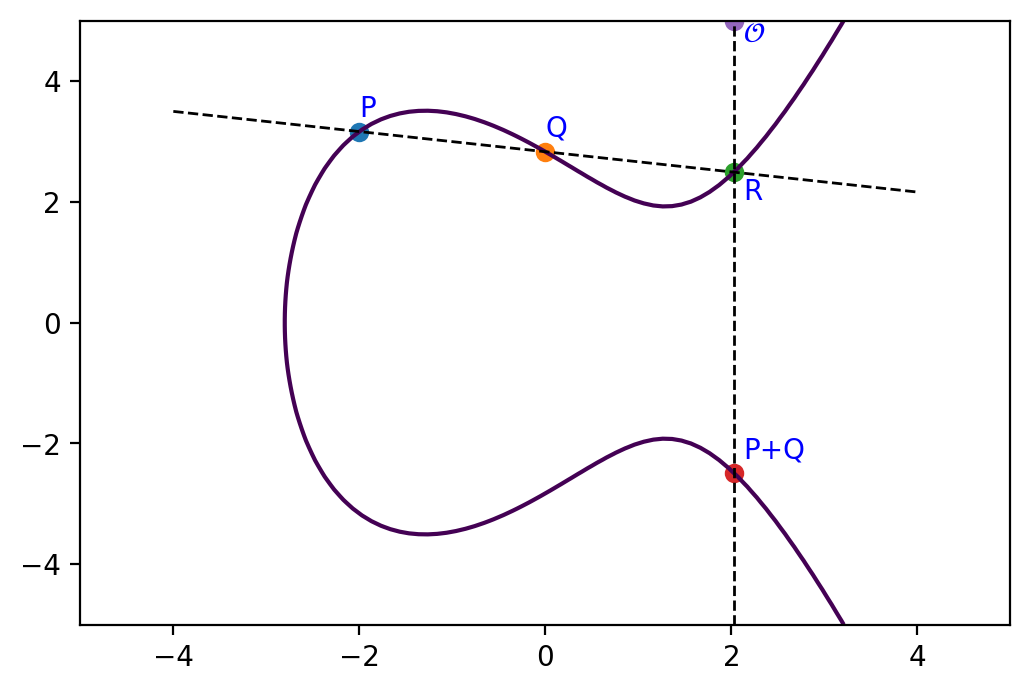
\includegraphics[width=.6\linewidth]{punktaddition.png}
    \caption{Punktaddition på $E$ se \ref{section:figur_2} for kode}
    \label{fig:geo_addition}
\end{figure}


Hvis vi kigger på \fref{fig:geo_addition} er punkterne $P, Q$ samt skæringspunktet $R$ indtegnet. Det inverse element af $R$ svarer til punktet symmetrisk om x-aksen. Vi har altså defineret følgende:
\begin{itemize}
	\item Elementerne for gruppen er punkter på den elliptiske kurve.
	\item Nulelementet er et punkt uendeligt langt væk: $\mathcal{O}$.
	\item Det inverse element for et punkt P er det som er symmetrisk om x-aksen.
	\item Addition er givet ved følgende regel. Givet tre skæringspunkter for en ret linje på en elliptisk kurve, da er deres sum lig med $P\oplus Q \oplus R=\mathcal{O}$.
\end{itemize}

Additionen af punkterne $P$ og $Q$ på \fref{fig:geo_addition} giver altså det inverse punkt af $R$ nemlig $-R$. Der er dog stadigvæk nogle tilfælde som der skal kigges på.

\begin{itemize}
    \item Hvad hvis $P=-Q$? I det her tilfælde vil sekantlinjen gennem de to punkter være vertikal og hermed ikke skære $E$ en tredje gang. Men hvis $P$ er den inverse af $Q$ har vi at. $P \oplus Q=Q \oplus (-Q)=\mathcal{O}$ fra definitionen om invertering se def. \ref{tab:definition_af_gruppe}.
    \item Hvad hvis punktet $Q=P$? Hvis $Q$ går mod $P$ har vi ikke længere en sekantlinje, men en tangent for kurven som vist på \fref{fig:tangent_addition}.
\end{itemize}


\begin{figure}[H]
    \centering
    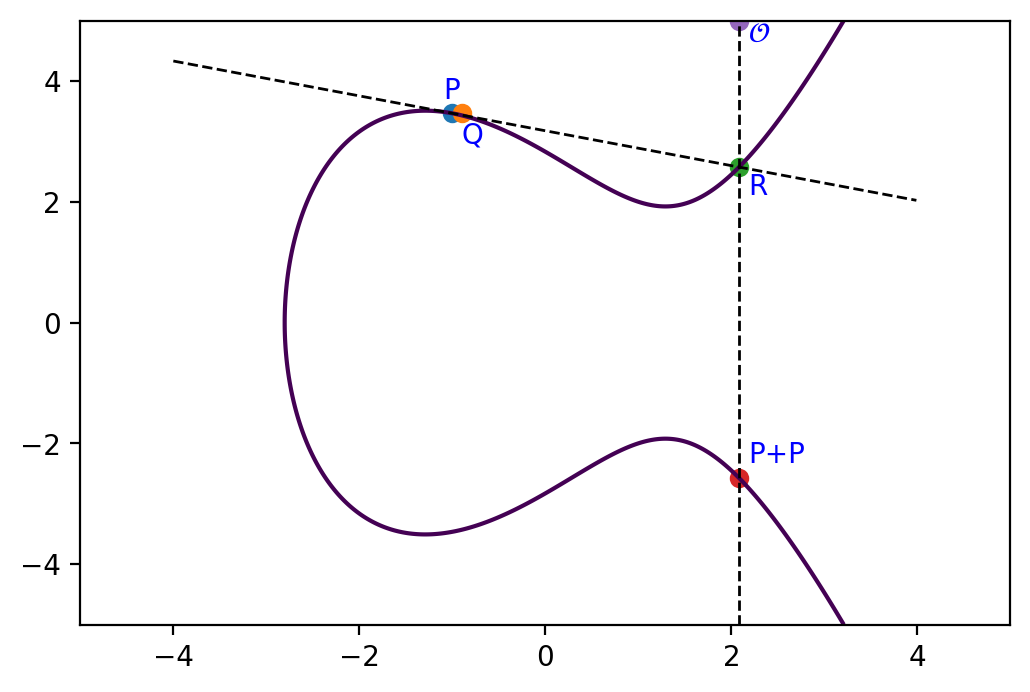
\includegraphics[width=0.7\linewidth]{tangent_addition.png}
    \caption{Punktaddition når $Q$ går mod $P$ se \ref{section:figur_3} for kode}
    \label{fig:tangent_addition}
\end{figure}

Som det kan ses på \fref{fig:tangent_addition} får vi altså at $P\oplus P=-R$ hvor $R$ er det anden skæringspunkt for tangenten.

\subsection{Algebraisk addition}
Hvis vi vil have en computer til at kunne lave overstående addition bliver vi nødt til at finde en algebraisk metode til at lægge punkterne sammen. Dette er også nødvendigt for at vise at definitionen for additionsformler på $E$ gælder (\cite{williamstein2006}) 

\begin{mdframed}[frametitle={Definition for additionsformler på $E$}]
Lad $P, Q$ være punkter på $E$ \fref{eq:ecc}. Det inverse element til $P$ er givet ved:
\begin{equation}\label{eq:invers}
    -P = (x_{P}, -y_{P})
\end{equation}
Ellers udføres additionen $P\oplus Q$ ved at beregne -R.

\begin{equation}
    a=
    \left\{\begin{matrix}\label{eq:slope}
     \frac{y_{P}-y_{Q}}{x_{P}-x_{Q}}& x_{Q} \neq x_P\\\\ 
     \frac{3x_{P}^2+A}{2\cdot y_{P}}& x_P = x_Q
    \end{matrix}\right.
\end{equation}

\begin{equation}
    x=a^2- x_P - x_Q
\end{equation}
\begin{equation}
    y=-a(x - x_P )- y_P
\end{equation}
\begin{equation}
    -R = (x, y)
\end{equation}


\end{mdframed}
Vi udleder nu definitionen for additionsformler på $E$. Vi ved at en ret linje er givet ved:
\begin{equation}\label{eq:ret_linje}
    L: \quad y=ax+b
\end{equation}
Samt ved vi at:
\begin{equation}\label{eq:ret_ligning}
    y = a(x-x_0)+y_0
\end{equation}
Når vi kender koordinaterne for punkterne $P$ og $Q$, kan vi finde hældningen og konstanten for den rette linje gennem punkterne ved:
\begin{equation}
    a = \frac{y_P-y_Q}{x_P-x_Q} \quad x_q \neq x_P
\end{equation}

\begin{equation}\label{eq:constant}
    b=y_P-a \cdot x_P=y_Q -a \cdot x_Q
\end{equation}

Skæringspunkterne mellem L: \fref{eq:ret_linje} og $E$ \fref{eq:E} må være givet ved løsningerne til ligningen:
\begin{equation}
    (ax+b)^2=x^3+Ax+B
\end{equation}

Indsætter \fref{eq:constant}.
$$(ax+y_P-a \cdot x_P )^2=x^3+Ax+B$$
$$(a(x - x_P ) + y_P )^2 = x^3 + Ax + B$$
$$a^2(x^2 + x_{P}^2 - 2x\cdot x_P ) + y_{P}^2 + 2axy_{P} - 2ay_{P}x_P = x^3 + Ax + B$$
\begin{equation}\label{eq:poly}
    \boldsymbol{-a^2} \cdot x_p^2 + 2\cdot a(ax+y_P)\cdot x_P + x^3 + Ax + ax^2 -2axy_P -y_p^2+B=0
\end{equation}
At finde en løsning til en tredjegradsligning kan være meget svært, men da vi kender to rødder ud af tre, kan vi bruge Vieta’s formel (\cite{youssefelhousni2018}).

\begin{mdframed}[frametitle={Vietas formel}]
Lad $P(x)=a_{n}x^n + a_{n-1}x^{n-1}+...+a_{1}x^1+ a_0$ være et polynomie af graden $n$ hvor $a_n \neq 0$. Der gælder da følgende sammenhæng mellem rødderne og koefficienterne:
\begin{equation}\label{eq:vietas}
    x_1 + x_2 + ... +x_n = \frac{-a_{n-1}}{a_n}
\end{equation}
\end{mdframed}

Vi ved at \fref{eq:poly} har tre rødder givet ved $x_P, x_Q$ samt $x_R$. Vi antager nu at roden vi gerne vil finde er $x_{R}$. Vi aflæser nu koefficienten til $x_{P}^2$ til at være $-a^2$. Hermed kan vi opskrive følgende.
$$ x_P + x_Q+x_R = \frac{-(-a^2)}{1} = a^2$$
$$ x_R = a^2- x_P - x_Q$$

Herefter får vi med ligningen for en ret linje \fref{eq:ret_ligning} at:
$$ y_R = a(x_{R}-x_{P})+y_{P} $$
Da $P\oplus Q=-R$ og vi ved at $-R$ er symmetrisk om x-aksen, må det svare til at gange y-koordinatet med $-1$.
\begin{equation}
    -R(x,y)=R(x,-y)
\end{equation}
Operationen for $P\oplus Q$ hvor $P \neq Q$ og punkterne er ikke symmetriske om x-aksen bliver da.
\begin{equation}
    x = a^2 -x_P -x_Q 
\end{equation}
\begin{equation}
    y = -a(x-x_P)-y_p
\end{equation}
\begin{equation}
    P\oplus Q=-R=(x, y)
\end{equation}

Hvor $a$ findes ved \fref{eq:slope}. Vi får dog et problem ved at finde hældningen med \fref{eq:slope} når $P=Q$. Som vi så tidligere gav dette tangenten til kurven $E$. Vi differentierer hermed $E$ ved brug af kædereglen.
$$f(x) = y = \pm \sqrt{x^3 + Ax +B}$$
$$ f'(x) = \pm \frac{3x^2 +A}{2\cdot \sqrt{x^3+Ax+B}}=\pm \frac{3x^2 +A}{2\cdot y}$$
Vi kigger kun på den positive løsning. Vi indsætter x-koordinatet for $P$ eller $Q$, finder vi hældningen $a$ når $x_P=x_Q$
\begin{equation}
    a = f'(x_Q)=f'(x_P)= \frac{3x_{P}^2 +A}{2\cdot y_P} \quad x_P \neq x_Q
\end{equation}

Vi dog stadigvæk anvende de samme formler for at finde $(x, y)$ som anvendt når $x_P \neq x_Q$. Hermed kommer vi frem til definitionen fra forrige afsnit og har hermed vist hvordan formlerne udledes. Det ses også at vi altid får et nyt punkt $-R$ som er en del af den elliptiske kurve da den altid er et skæringspunkt, hvilket gør at vores gruppe er lukket. 

\subsection{Associativitet}
Det eneste vi mangler for at have vist at vores gruppe overholder kriterierne for en gruppe er at den er assosicativ altså $a\oplus(b\oplus c)=(a\oplus b)\oplus c$. Der er et bevis for associativiteten for en gruppe på en elliptisk kurve, men da det mest simple bevis jeg var i stand til at finde fylder ca. 9 sider og bliver betegnet som \textit{"rather messy"} undlader jeg at gennemgå dette. Se (\cite{stefanfriedel2017}) for bevis. I stedet prøver jeg at komme med et logisk argument. 
Hvis vi har punkterne $P,Q,R$ som alle ligger på en ret linje ved vi, at deres orden er ligegyldig betydende, at hvis to punkter går igennem den linje vi laver vil det tredje punkt også. Dette  betyder at hvis alle punkter ligger på en ret linje, må $P\oplus (Q\oplus R)=Q\oplus (P\oplus R)=...=\mathcal{O}$. 

\section{Skalarmultiplikation}
I følgende afsnit introduceres begrebet \textit{skalarmultiplikation}. Udover at kunne lægge punkter sammen en af gangen, opstiller vi en operation til at kunne ligge et punkt \textit{n gange} til sig selv. Vi bruger skalarmultiplikation givet ved:
\begin{equation}
    n \cdot P =\underbrace{P\oplus P\oplus P\oplus ...\oplus P}_\text{n gange}
\end{equation}
Ligesom tidligere som for $\oplus$ er gangetegnet altså ikke en \textit{normal} operation, men i stedet en vi definerer.
Når man kigger på overstående tænkes det at $n \cdot P$ kræver $n$ additioner af punkter altså $O(n)$ i tidskompleksitet. Dette bliver meget hurtigt rigtigt langsomt når $n$ bliver stort Vi kan dog bruge en algoritme som hedder \code{double-and-add} (\cite{andreacorbellini2015}). Vi sætter $n=151$ som eksempel, der ved binær er givet ved $10010111_2$:
$$151=2^7+2^4+2^2+2^1+2^0$$
Hvilket giver:
$$151\cdot P=2^7 \cdot P \oplus 2^4 \cdot P \oplus 2^2 \cdot P \oplus 2^1 \cdot P \oplus 2^0 \cdot P$$
Måden dette udregnes på er så ved at kigge på det binære tal og gå iterativt igennem bits'ne i det. Hvis det enkelte bit er lig med $1$ laver man en addition efterfulgt af en dublering. Hvis det enkelte bit i stedet er lig med $0$ laves der kun en dublering. For overstående får vi altså:
\begin{itemize}
    \item Tag $P$
    \item Dubler $P$ og få $(2\cdot P)$
    \item Lig $2\cdot P$ til $P$
    \item Dubler $2\cdot P$ og få $(2^2 \cdot P)$
    \item osv...
\end{itemize}
Ved brug af overstående metode kan vi udregne $151 \cdot P$ ved bare $7$ dubleringer og $4$ additioner. I implementeringen kan pseudokoden for algoritmen ses i \fref{sec:skalarmultiplikation}, mens koden kan findes i bilaget se \fref{sec:code}. Det vigtigste at tage med er dog at vi i stedet for $O(n)$ reducerer tidskompleksiteten til $O(log_2 n)$, da algoritmen er "lineær" i forhold til længden af det binære tal.



\section{Elliptiske kurver over endelige legemer}
At bruge alle de reele tal er ikke smart, når vi gerne vil have en computer til at lave diverse operationer. I nogen tilfælde, kan vi få punkter med rigtigt mange decimaltal, som skal beskrives helt nøjagtigt for at vores addition virker. Udover det er det meget svært at regne på uendeligheder, og vi har derfor brug for en \textit{finit} mængde. For at få en finit mængde opstiller vi i stedet vores gruppe som et endeligt legeme, som indeholder en finit mængde elementer. Først introducerer vi dog begrebet moduloregning.

\subsection{Modulær aritmetik}
Modulær aritmetik eller moduloregning er i sin mest elementære form aritmetik, som nulstiller sig selv hver gang et bestemt heltal \textit{N} er nået. Et kendt eksempel på moduloregning er et 12-times ur, hvor dagen er inddelt i to 12-timers perioder. Hvis klokken er 7:00 så vil den $8$ timer senere være 3:00. Hvis vi ligger tallene sammen får vi $7+8=15$, men da klokken "nulstiller sig selv" hver 12 time giver det hermed $3$. Et 12-timers ur er altså \textit{modulo 12}. Vi opskriver det som:
$$7+8 \equiv 3 \pmod{12}$$
Man kan sige at 3 er resten ved at dividere 15 med 12.

\subsection{Endelige legemer for elliptiske kurver}
Det endelige legeme vi vil anvende, er alle heltal modulo $p$, hvor $p$ er et primtal. Vi kalder denne mængde af tal for $\mathbb{F}_p$. Indtil videre har vi brugt \fref{eq:ecc} men den ændres nu til.

\begin{mdframed}[frametitle={Endeligt legeme for elliptisk kurve}]
\begin{equation}\label{eq:ecc_finite}
    \{(x,y) \in \mathbb{F}_{P}^2\ | \quad y^2 \equiv x^3+Ax+B \pmod{p}, 4A^3 + 27B^2 \not\equiv 0 \pmod{p} \} \cup \{\mathcal{O}\}
\end{equation}
\end{mdframed}

Hvor $\mathcal{O}$ stadigvæk er punktet ved uendelig, samt at $A$ og $B$ er heltal i $\mathbb{F}_{p}$. Dette former en ny gruppe over $\mathbb{F}_p$ hvor additionslovene er de samme som tidligere. I stedet for graferne for elliptiske kurver som vist tidligere, fås følgende når vi plotter.

\begin{figure}[htbp]
\centering
\begin{subfigure}{.5\textwidth}
  \centering
  \includesvg[width=1.1\linewidth]{finite_mod_37.svg}
  \caption{$p=37$}
  \label{fig:sub1}
\end{subfigure}%
\begin{subfigure}{.5\textwidth}
  \centering
  \includesvg[width=1.1\linewidth]{finite_mod_487.svg}
  \caption{$p=487$}
  \label{fig:sub2}
\end{subfigure}
\caption{Afbildning af den elliptiske kurve $y^2 \equiv x^3-5x+8 \pmod{p}$. Se \ref{section:figur_4} for kode}
\label{fig:finit_felt}
\end{figure}

Ovenover ses \fref{fig:finit_felt} for en elliptisk kurve som er kongurent med $p$. Bemærk at der maksimalt for hvert $x$ kun er to punkter. Udover det er ingen punkter på graferne større end $p$ grundet at vi tager modulo $p$ på dem. Som det kan ses ser vores figur meget anderledes ud hvis man sammenligner dem med tidligere. Vi kan dog stadigt lave samme geometriske additioner. Da det er et endeligt legeme vi regner over, kan vi ikke dividere normalt, da division svarer til at tage den modulære multiplikative inverse. Det svarer til at løse ligningen:
\begin{equation}\label{eq:division}
ax \equiv 1 \pmod{p}
\end{equation}

Hvor $x$ er den modulære multiplikative invers. Sagt med andre ord er resten af at dividere $a\cdot x$ med et heltal $p$ lig med $1$. Med euklids udvidede algoritme, kan vi dog hurtigt udregne overstående ligning (\cite{donaldknuth1968}).


\section{Anvendelse af elliptiske kurver i kryptologi}
At bruge tal- og gruppeteori til forskellige krypteringsalgoritmer, er et af de mest populære konkrete eksempler på hvordan denne type af matematik kan bruges. Det er også en af de vigtigste emner indenfor matematik i nyere tid, da det ligger til grund for alt digitalt lige fra banker til hjemmesider. Med punkter på elliptiske kurver, kan vi altså sikre det meste af internettet fra tredjemænd i at kunne kigge med!

\subsection{Assymetrisk kryptering}
Assymetrisk- eller public-key kryptering betegner et system hvor alle parter har en offentlig- og en privat nøgle (\cite{seanriley2017}). Den offentlige nøgle, må alle parter i systemet kende til, mens den private nøgle holdes hemmelig. For overskuelighedens skyld kalder vi de to parter i systemet for Alice og Bob.

I et assymetrisk kryptosystem kan Bob og Alice sende krypterede beskeder til hinanden ved brug af hinandens offentlige nøgler uden at en tredjepart kan læse dem. Den eneste måde for en tredjepart at læse deres beskeder vil være ved at finde ud af hvad deres private nøgler er. Der findes mange forskellige algoritmer til assymetrisk kryptering. Jeg har dog valgt at kigge nærmere på \code{Elliptic-Curve Diffie-Hellman key exchange}. 

\subsubsection{Public-Key Exchange - ECDH}
Elliptic-Curve Diffie-Hellman key exchange er en måde til at kombinere Alice og Bob’s public keys sammen således at man får en ny nøgle der kan udføres symmetrisk kryptering med. test

\begin{figure}[htbp]
\centering
\begin{subfigure}{.5\textwidth}
  \centering
  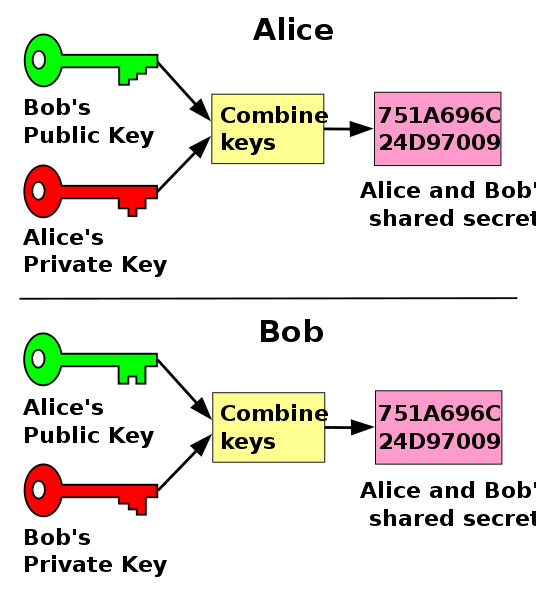
\includegraphics[width=0.9\linewidth]{images/Public_key_shared_secret.svg.png}
  \caption{(\cite{gothberg_2006})}
  \label{fig:sub1}
\end{subfigure}%
\begin{subfigure}{.5\textwidth}
  \centering
  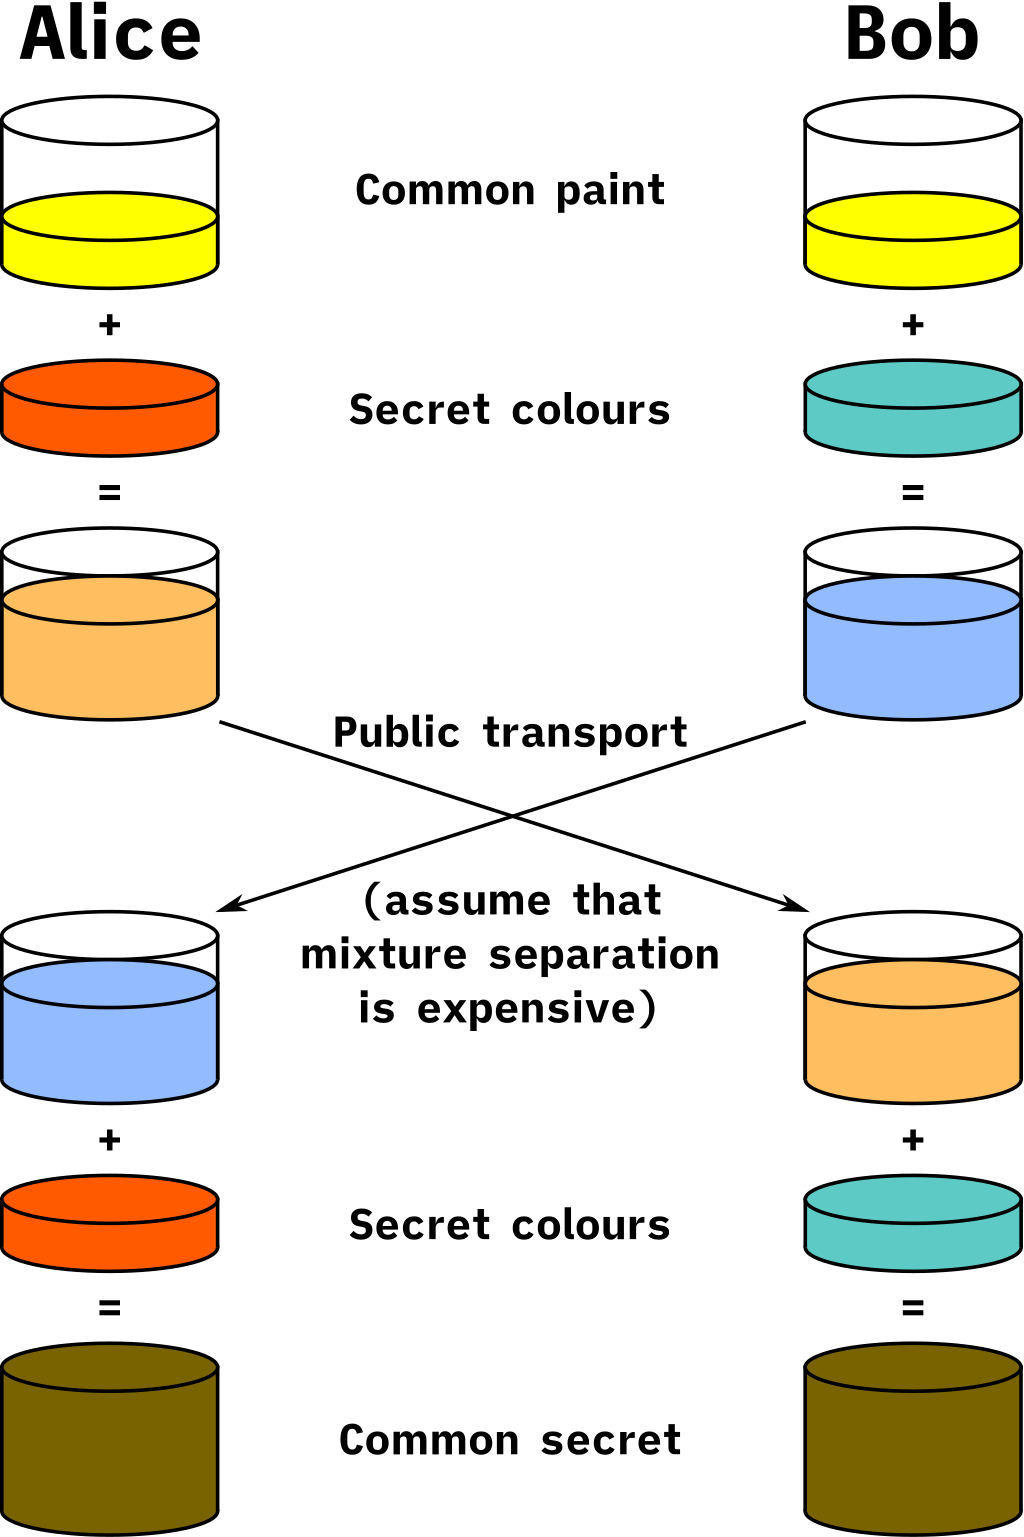
\includegraphics[width=0.7\linewidth]{images/1024px-Diffie-Hellman_Key_Exchange.svg.png}
  \caption{(\cite{Avinck_2011})}
  \label{fig:sub2}
\end{subfigure}
\caption{Illustration af Diffie-Hellmann key Exchange}
\end{figure}

På overstående figurer ses to forskellige måder til at vise hvordan et Diffie-Helmann key exchange hænger sammen. Vi kigger først på figuren til højre. Alices private nøgle vil være den mørkeorange, mens hendes offentlige nøgle er den lyse orange. Hun sender nu sin lyse orange farve til Bob som kombinerer den med sin private nøgle og får: \code{(orange+gul)+turkis=fælles hemmelighed}. Det samme kan Alice gøre: \code{(turkis+gul)+orange=fælles hemmelighed}. Vi får den samme hemmelighed, da operationen er associativ. Hermed er der udført et key-exchange som parterne hver især nu kan bruge til symmetrisk kryptering og sende beskeder til hinanden. Dette kunne eksempelvis gøres med AES-kryptering. Vi kigger nu mere teknisk på hvordan det fungerer i forbindelse med elliptiske kurver \code{ECDH}.
\begin{table}[h]
\label{tab:key_exchange}
\begin{tabular}{|l|l|l|}
\hline
\textbf{Alice}                                                                                                                                                          & \textbf{Public Space}                                                                                                                                                  & \textbf{Bob}                                                                                                                                                       \\ \hline \hline
\begin{tabular}[c]{@{}l@{}}Alice vælger sin private nøgle \\ ved at tage et tilfældigt heltal \\ mellem $1 \leq \alpha \leq n-1$. \\ Privatnøgle $=\alpha$\end{tabular} & \begin{tabular}[c]{@{}l@{}}$p$ primtal\\ $A, B$ koefficienter til den\\ elliptiske kurve\\ $G$ generatorpunktet\\ $n$ ordenen (antal punkter i\\ legemet)\end{tabular} & \begin{tabular}[c]{@{}l@{}}Bob vælger sin private nøgle\\ ved at tage et tilfældigt heltal \\ mellem $1 \leq \alpha \leq n-1$.\\ Privatnøgle $=\beta$\end{tabular} \\ \hline
\begin{tabular}[c]{@{}l@{}}Udregner nyt punkt ved \\ skalarmultiplikation:\\ $$ A = \alpha \cdot G$$\end{tabular}                                              &                                                                                                                                                                        & \begin{tabular}[c]{@{}l@{}}Udregner nyt punkt ved \\ skalarmultiplikation:\\ $$ B = \beta \cdot G$$\end{tabular}                                          \\ \hline
Modtager $B=(x_B, y_B)$                                                                                                                                                  & \begin{tabular}[c]{@{}l@{}}$A=\alpha \cdot G = (x_A, y_A)$\\ $B = \beta \cdot G = (x_B, y_B)$\end{tabular}                                                                         & Modtager $A=(x_A, y_A)$                                                                                                                                             \\ \hline
\begin{tabular}[c]{@{}l@{}}Udregner nyt punkt ved\\ skalarmultiplikation:\\ $P=\alpha \cdot B= \alpha \cdot (\beta \cdot G)$\end{tabular}                                                   &                                                                                                                                                                        & \begin{tabular}[c]{@{}l@{}}Udregner nyt punkt ved\\ skalarmultiplikation:\\ $P=\beta \cdot A = \beta \cdot (\alpha \cdot G)$\end{tabular}                                              \\ \hline
\end{tabular}
\caption{Gennemgang af ECDH: Elliptic Curve Diffie-Helmann key-exchange}
\label{tab:key_exchange_diffie}
\end{table}
\FloatBarrier
Hermed har Alice og Bob fået en fælles nøgle, som de kan bruge til at kryptere beskeder med. 
Bemærk at hvis MITM \textit{(man in the middle)} skal kunne finde frem til $P$ kræver det at de enten kender $\alpha$ eller $\beta$. Umiddelbart kunne det tænkes, at man kan løse udtrykket $\alpha = \frac{A}{G}$, men da $G$ er et element kan vi ikke dividere på denne måde, da division bliver til det inverse element og hermed et helt andet punkt. 

\section{Det diskrete logaritmeproblem}
I følgende afsnit redegøres der for det diskrete logaritmeproblem, hvorefter en algoritme til at løse problemet opstilles. Efter dette sammenlignes tidsforbruget af algoritmen med tiden for at generere en offentlig nøgle. 

Hvis MITM vil bryde krypteringen, går det ud på at løse det nedenstående problem.
\begin{mdframed}[frametitle={Det diskrete logaritmeproblem for elliptiske kurver}]
Givet to punkter $A$ og $G$ find heltallet $\alpha$ som opfylder ligningen:
\begin{equation}
    A=\alpha \cdot G
\end{equation}
Hvor $\alpha$ er et helt tal og $G$ og $A$ er gruppeelementer.
\end{mdframed}

Dette problem kaldes for: Det diskrete logaritmeproblem for ECC og siges at være et \textit{”svært problem”}, da der ikke findes nogen algoritme som kan løse det på en bestemt polynomisk tid, som kan køre på en \textit{”normal”} computer (\cite{youssefelhousni2018}). Det er dog vigtigt at sige, at der ikke til dags dato, findes et bevis for at forrige postulat er sandt (\cite{timsroberts}). Umiddelbart har navnet: Det diskrete logaritmeproblem ingen sammenhæng med elliptiske kurver, men det skyles at det stammer fra andre grupper hvor man i stedet bruger \textit{multiplikativ} notation hvor ligningen opskrives som $A=G^\alpha  \pmod{p}$. Her skriver vi løsningen  som $log_{G}A=\alpha$. Vi kigger nu på gruppen for $Z_p \backslash {0}$ hvor $p$ er et stort primtal. Vi ved at den har $p-1$ elementer. At lave en algoritme til at løse dette problem er ikke særligt svært, da vi skal udregne $2G, 3G, 4G$ indtil at et af dem bliver lig med $A$.
\\\\
\begin{python}
	def brute_force(G, public_key, p):
		temp_point = G
		for i in range(1, p):
			if temp_point == public_key:
				return(i)
			temp_point = mult(i+1, G)
\end{python}
Overstående algoritme går iterativt igennem alle heltal fra 1 til $p$ indtil at $iG$ er lig med den offentlige nøgle.
Algoritmen vil stoppe efter $log_{G}A$ iterationer, og vi kan hermed løse problemet forholdsvist nemt til tiden $O(n)$, hvor $n$ er ordenen af $G$. Da en computer kan udføre ekstremt mange operationer meget hurtigt, kan vi kun bruge grupper med rigtigt store ordener. Vi kan fx, kigge på hvis $n > 2^{100}$, svarende til et tal som er 100 bit langt. Vi antager nu at en computer kan lave 1 milliard operationer svarende til ca. $2^{30}$ operationer pr sekund. Vi får at det vil tage $3,75\cdot 10^{13}\cdot$ år altså over 1 billion år at udregne $2^{100}$. Denne \textit{”brute-force”} algoritme kan altså ikke anvendes i praktisk når $n > 2^{100}$.


Hvad så med den anden vej når vi skal udregne $\alpha \cdot G$? Dette er ikke svært grundet vores double-and-add algoritme som tidligere beskrevet, hvor vi reducerer tiden til $O(log_{2}n)$ i stedet for $O(n)$. I praksis vil det sige at hvis Alice og Bob vælger at lave deres private key en bit længere, skal de kun udføre to ekstra regneoperationer hver \textit{(double-and-add)}, mens MITM som prøver at bryde krypteringen skal bruge dobbelt så meget regnekraft pr. ekstra bit.


Det kan hermed ses at krypteringen vokser lineært i forhold til bitlængden $k$, hvor arbejdet ved at løse det diskrete logaritmeproblem i gruppen stiger eksponentielt med bitlængden. Til at vise følgende også gælder for virkeligheden, har jeg implementeret brute-force metoden i mit program. Ved at iterere over forskellige privat-nøgler med en step-size på $2^i$ kan vi lave et plot med bitlængden af privatnøglen samt tiden det tog at udregne. Python-biblioteket \code{timeit} blev anvendt

\begin{figure}[htbp]
\centering
\begin{subfigure}{.5\textwidth}
  \centering
  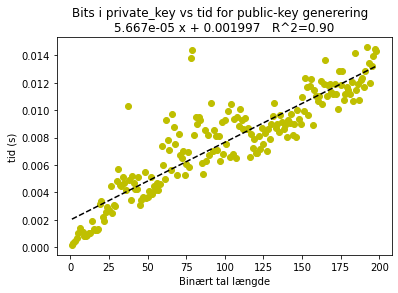
\includegraphics[width=1.0\linewidth]{images/gen.png}
  \caption{Public-Key generering (Double-and-Add)}
  \label{fig:sub1}
\end{subfigure}%
\begin{subfigure}{.5\textwidth}
  \centering
  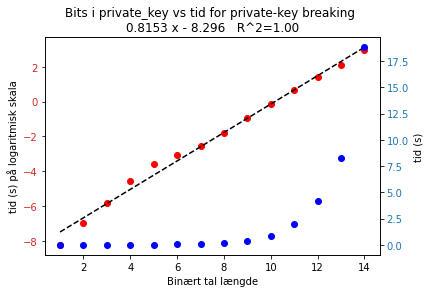
\includegraphics[width=1.0\linewidth]{images/breaking.png}
  \caption{Private-Key breaking (Naiv algoritme)}
  \label{fig:sub2}
\end{subfigure}
\caption{Modellering af generering vs. breaking af nøgler se \ref{section:figur_6} for kode}
\label{fig:genvsbreak}
\end{figure}

På \fref{fig:genvsbreak}a ses et punktplot af længden af privatnøglens længde i binær udaf førsteaksen, og tiden det tog at udregne på andenaksen. Udover det er der foretaget en lineær regression, hvor vi får modellen: $t_{gen}=5,667\cdot 10^{-5}\cdot k + 1,997\cdot 10^{-4}$ hvor $k$ er længden af det binære tal. Da vi får en $R^2=0,90$ kan vi konkludere at vores model er valid. Det kan dog ses at der generelt kommer en større afvigelse fra modellen når længden af det binære tal stiger. Vi udregner nu tiden det ville tage for en 100-bit lang private-key.
$$t_{gen} (100)=5,667\cdot 10^{-5}\cdot 100 + 1,997\cdot 10^{-4}=0,006$$
Hermed vil det ifølge vores model tage ca. 0,006 sekunder at generere en public-key som er 100 bit lang. 


På \fref{fig:genvsbreak}b ses et punktplot for tiden det tager at finde private-key ud fra public-key. Bemærk at den røde dataserie er på en logaritmisk skala. Ved at lave en lineær regression på den logaritmiske skala fås modellen: $t_{break}=8,153 \cdot 10^{-1} \cdot k-8,296$ med en $R^2=1,00$. Vi kan hermed udregne tiden det vil tage for en 100 bit lang private-key.

$$t_{break}(100)=8,153 \cdot 10^{-1} \cdot 100 - 8,296 = 73,53$$
Omregner fra logaritmisk skala.
$$e^{73,53}=8,58\cdot 10^{31}$$
Hvis vi omregner $8,58\cdot 10^{31}\cdot$s til år fås $2,72 \cdot 10^{24}\cdot$år, hvilket er så lang tid at det næsten er umuligt at forholde sig til. Bemærk at programmet blev kørt på en laptop (\textit{Lenovo X1 Carbon 6th gen I7}) hvilket gør at eksikveringstiden er meget langsom i forhold til en supercomputer. Ligeledes er koden skrevet i Python, som er et forholdsvist langsomt kodesprog.  

Der findes algoritmer såsom \textit{Shanks: ”Baby steps, Giants steps”} algoritme, som på en smart måde kan nedbringe tidskompleksiteten i forhold til vores naive brute-force algoritme så den ikke er eksponentiel, men det er her elliptiske kurvekryptografi kommer ind. Når vi kigger på det diskrete logaritmeproblem i forhold til ellipitiske kurver, findes der ikke til dags dato specialiserede algoritmer som virker på disse typer af grupper, undtagen specifikke kendte kurver, hvilket gør at private key-længden kan være kortere i praksis sammenlignet med mange andre kryptosystemer. Det er endda vist at chancen for at man finder en sådan algoritme er højst usandsynlig (\cite{Ramachandran}).
\section{Implementering}
I følgende afsnit implementeres et elliptisk kurvekryptosystem til at udføre kryptering. Herefter vises et eksempel på en key-exchange, hvorefter sikkerheden i det implementerede system diskuteres.

\subsection{Valg af programmeringssprog}
Da kryptering er noget man gerne vil have sker hurtigst muligt, giver det bedst mening hvis det skal anvendes i industrien at bruge sprog såsom C eller C++. Jeg har dog valgt at lave mit program i python, da python understøtter heltal af arbitrær størrelse, hvilket C eller C++ ikke gør. Dette gør at koden bliver meget nemmere at skrive og forstå. 

\subsection{Valg af kurve}
Når vi skal lave en implementering i praksis, er det vigtigt at vælge en ”sikker” elliptisk kurve. Nogen kurver kan nemlig blive udsat for forskellige angreb, som det diskuteres mere i vurderingen af systemet. En af de mest kendte sider til at finde kurver på er safecurves.cr.yp.to, som laver store mængder forskning ifb. med forskellige typer af angreb på deres kurver inden de anbefales. Ud fra hjemmesiden vælger jeg kurven M-221, da den er verificeret som sikker (\cite{danielj.bernsteintanjalange2014}). Den har parametrene givet ved:
\begin{python}
# M-221 https://eprint.iacr.org/2013/647.pdf
p = 0x1FFFFFFFFFFFFFFFFFFFFFFFFFFFFFFFFFFFFFFFFFFFFFFFFFFFFFFD
A = 0x01c93a
B = 0x01
G = (0x04, 0x0f7acdd2a4939571d1cef14eca37c228e61dbff10707dc6c08c5056d)
n = 0x040000000000000000000000000015A08ED730E8A2F77F005042605B
\end{python}
Bemærk at talet er skrevet i hex, som det kan ses på præfiks givet ved $0x$

\subsection{Addition på elliptisk kurve}
For at kunne oversætte matematikken til kodning, skal vi ud fra vores endelige legeme fremstille en algoritme for additionsformlerne se definition. Hermed kan vi opskrive følgende (\cite{williamstein2006}):

\begin{algorithmic}

\If{$P_1 = \mathcal{O}$ or $P_2 = \mathcal{O}$} 
    \State \Return $P_3 = \mathcal{O}$
    \EndIf
\If{$x_1 = x_2 $ and $ y_1 = -y_2 $}
    \State \Return $P_3 = \mathcal{O}$
    \EndIf
\If{$P_1 = P_2$}
    \State $a \gets \frac{3x_{1}^2+A}{2\cdot y_{1}}$
\Else
    \State $\frac{y_{P}-y_{Q}}{x_{P}-x_{Q}}$
\EndIf
\State $x_3 \gets a^2 - x_1 - x_2$
\State $y_3 \gets -a(x_{3}- x_1 )- y_1$
\State \Return $(x_3, y_3)$

\end{algorithmic}

Da punktet $\mathcal{O}$ er et irrationelt tal, kan vi ikke regne med det på en computer. Vi definerer hermed \code{None} til at være lig med $O$ i koden. Bemærk også at ved division menes at tage den modulære multiplikative inverse som findes ved Euklids udvidede algoritme. Denne algoritme er implementeret via (\cite{andrewharrington}), hvorefter den er modificeret til \textit{kun} at returnere den modulære multiplikative inverse.

\subsection{Skalarmultiplikation}
\label{sec:skalarmultiplikation}
Vi opstiller nu pseudo-kode for algoritmen for skalarmultiplikation hvor n er antal gange til at addere og P er et punkt.
\\
\begin{algorithmic}
    \State def $mult(n, P)$

    \If{$n = n_E$}    \Comment{$n_E$ the order of the curve}
        \State \Return $\mathcal{O}$
    \ElsIf{$n < 0$}
        \State \Return $mult(-n, P)$ \Comment{run algorithm again with $-n$}
    \EndIf
    \State $new\_point \gets \mathcal{O}$
    \State $temp\_point \gets P$

    \While{$n$} \Comment{Continue until is false ($n=0$)}
        \If{$n \& 1 = true$} \Comment{Get first binary digit}
        \State $new\_point \gets new\_point + temp\_point$
        \EndIf
        \State $temp\_point \gets double(temp\_point)$ \Comment{same as P+P}
        \State $n \gets n>>1$ \Comment{Right shift binary number}
    \EndWhile
    \State \Return $new\_point$
\end{algorithmic}

Når der står \code{while n}, menes der at algoritmen vil fortsætte indtil det binære repræsentation for tallet n er lig med 0. Når der står at der foretages et right shift menes der at det tallet \code{1001} bliver til \code{100}, vi fjerner altså det første bit af tallet. 

\subsection{Hjælpefunktioner}
Udover at have addition og skalarmultiplikation er der en række andre hjælpefunktioner. Dette inkluderer bla. Andet \code{discriminant} som returnerer om ellipsen er valid for elliptisk kurvekryptografi. Funktionen \code{is\_on\_curve} returnerer \code{True} hvis punktet som er givet er på kurven, hvilket er smart til at tjekke udregninger. 

\subsection{Diffie-Hellmann key exchange eksempel}
For at lave et Diffie-Helmann key exchange bruger vi algoritmen som forklaret i \fref{tab:key_exchange_diffie}. Nedenunder ses et konkret eksempel på hvordan det laves. Først genererer Alice og Bob deres private og public keys. Bemærk \code{e} er et objekt for klassen \code{EllipticCurve} med \code{M-221}.
\begin{python}
# generate private keys
a = random.randint(1, p-1)
b = random.randint(1, p-1)

# generate public keys
A = e.mult(a, G)
B = e.mult(b, G)
\end{python}
Nu kan vi udregne deres shared secret:
\begin{python}
# Shared secret from other person public key
a_shared_secret = e.mult(a, B)
b_shared_secret = e.mult(b, A)

#check if keys are the same
assert a_shared_secret == b_shared_secret
print(a_shared_secret)
\end{python}
\code{> (E95FB24B62D35FDAE41997349B662AC4B71432A50408ADED7D5F21F, \\ 1F8A09D24045BF379EE29BFCC6D8A12271DED95E8691934F442ACFAA)}

Da begge deres secrets var den samme, kan vi konkludere at de har fået et \code{keypair} ved brug af hinandens \code{public\_keys}. I praksis anvender man kun $x$-koordinatet for ens secret, for at gemme mindre data.

\subsection{Sikkerheden i det implementerede system}
Som analyseret tidligere er krypteringen meget svær at bryde. Dog er der mange andre typer af angreb man kan lave. Problemet med et Diffie-Helmann key exchange er, at det kræver at man stoler på at den man kommunikerer med, ikke udgør sig for at være en anden. 
\begin{figure}[htbp]
    \centering
    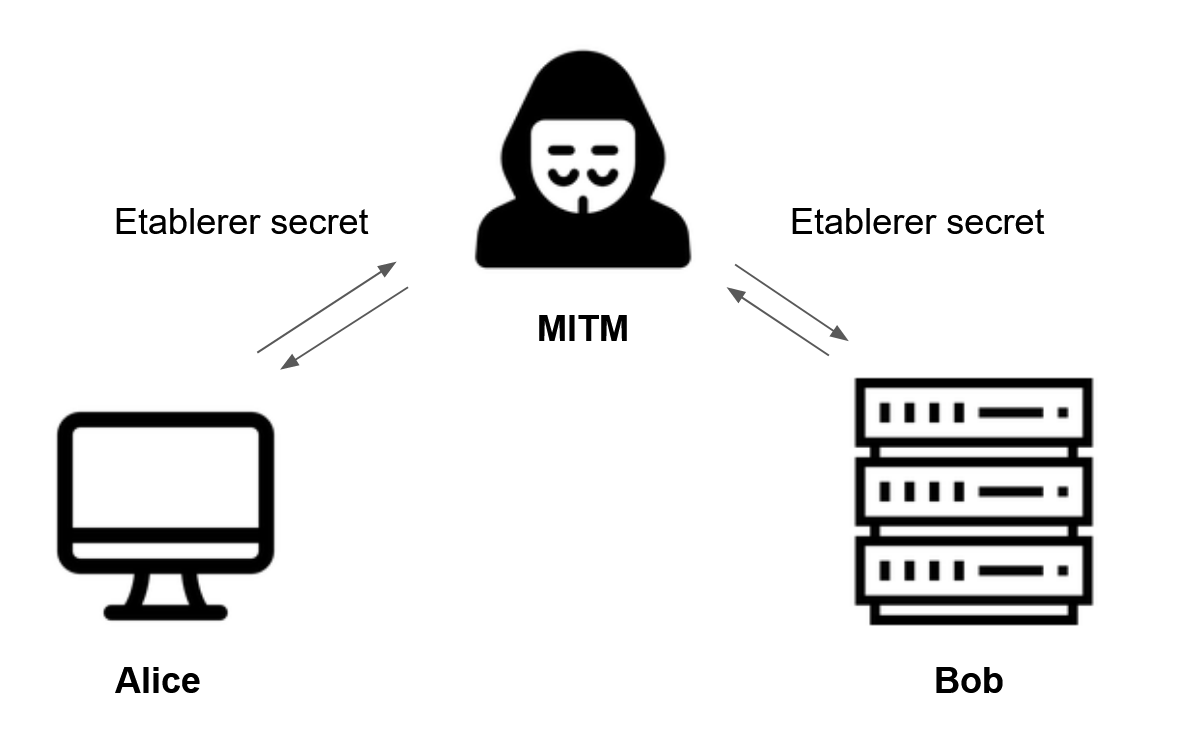
\includegraphics[width=0.6\linewidth]{images/MITM.png}
    \caption{MITM som udgiver sig for at være en anden}
    \label{fig:MITM}
\end{figure}
\FloatBarrier

Som det ses på \fref{fig:MITM}, kan MITM som oftest er en proxy udgive sig for at være en anden. Når Alice (computeren) sender en besked krypterer hun den med en public key som er en anden end den Bob har. MITM kan nu dekryptere beskeden og kryptere den igen med hans fælles secret med Bob (\cite{seanriley12017}). 

En måde at undgå et sådan angreb er ved at implementere en digital signatur som beviser at det er hende som har foretaget krypteringen. Bob kan hermed se at den secret key han modtager ikke kan være blevet ændret i. Eksempler på disse systemer er fx ECDSA (\cite{youssefelhousni2018}). 
Det kan hermed ses at sikkerheden i forhold til krypteringen er meget sikker i det implementerede system, men der er andre typer af angreb, som gør at systemet ikke kan anvendes i praktisk medmindre man er helt sikker på at ens kommunikation ikke er komprimeret. 

\section{ECC, et alternativ til RSA-kryptering?}
RSA var det første public-key kryptosystem som blev adopteret af mange internetprotokoller. Systemet er bedre end et klassisk diffie-helmann key exchange, da man kan lave signaturer. Dog er det blevet vist, at nogle algoritmer kan løse det diskrete logaritmeproblem på under eksponentiel tid for RSA (\cite{carlpomerance1987}). I forbindelse med, at computere er blevet meget hurtigere har RSA-nøglers længde været nødt til at følge med. Dette har gjort, at RSA-kryptering er blevet langt tungere på mindre enheder såsom IOT, hvor kryptering er meget vigtigt \cite{nilsguraarunpatel2004}. 

\begin{table}[htbp]
\centering
\begin{tabular}{lll}
\toprule
\textbf{Security Bit Level} & \textbf{RSA} & \textbf{ECC} \\ \midrule
80                          & 1024         & 160          \\ 
112                         & 2048         & 224          \\ 
128                         & 3072         & 256          \\ 
192                         & 7680         & 384          \\ 
256                         & 15360        & 512          \\ 
\bottomrule
\end{tabular}
\caption{\cite{mahto}}
\label{tab:RSAvsECC}
\end{table}


\FloatBarrier
På overstående \fref{tab:RSAvsECC} ses en data fra NIST \textit{(National Institute of Standards and Technology)} over den anbefalede sikkerhed ift. bitlængde. Som det kan ses, er key-længden for RSA kraftigt stigende hvor ECC er noget kortere. Ved 256-bit sikkerhed skal en RSA-key være 15360 bit lang (1,92 kB), hvor ECC kun skal være 512 bit. Selvom 1,92 kB ikke er meget, kan en server med mange tusinde requests hurtigt fylde meget plads op. 
\\\\
Det kan hermed ses at hvis man kigger på sikkerheden bag systemerne ift. kryptering, er ECC langt mere effektivt end RSA. Dog har ECC også haft sine egne udfordringer. Et af de større problemer ved ECC, er at man skal blive enige om at bruge en specifik kurve. Man har igennem årene prøvet at lave databaser såsom safecurves.cr.yp.to, men selv disse ”uafhængige” parter er blevet beskyldt for ikke at være klare i alt deres forskning ift hvad de mener er en ”god kurve” (\cite{satoshinichi2020}). En del af Edward Snowdens læk af fortrolige dokumenter i 2013 inkluderede at NSA havde betalt en gruppe problemløsere 10 millioner USD for at indbygge en Kleptografisk\footnote{Et kleptografisk angreb, bruger asymmetrisk kryptografi til at implementere en kryptografisk bagdør der er svær at finde.\cite{patrickvacek2013}} bagdør i \textit{(Dual\_EC\_DRBG)} brugt til at generere pseudotilfældige tal (\cite{josephmenn2013}). Efter denne begivenhed er der kommet langt større fokus på at sikre sig at kurver er sikre, men i forhold til RSA-kryptering er det en ulempe at skulle anvende så mange offentlige parametre. \\\\
Det er i det hele taget vigtigt at huske, at det indtil videre har været umuligt at bevise at det diskrete logaritmeproblem både for RSA og elliptiske kurver ikke kan løses med en meget hurtig algoritme på en almindelig computer. Kvantecomputere vil også i fremtiden blive en reel trussel til public-key kryptering. Selvom kvantecomptutere i dag er meget teoretiske er der store organisationer såsom NSA der forsker meget i hvordan de kan implementeres (\cite{nsa2022}). Når kvantecomputere kan arbejde med et reelt antal qubits\footnote{En \textit{"qubit"} (eller \textit{"kvantebit"}) er den kvantemekaniske analog til en klassisk bit.} vil det blive enden på kryptografi som vi kender det i dag. Shors’ algoritme på en kvantecomputer er nemlig blevet vist til at kunne løse det diskrete logaritmeproblem for en abelsk gruppe på en elliptisk kurve. For at kunne undgå dette, er meget forskning lige nu i gang med at undersøge om man i stedet kan bruge ikke-abelske grupper som Shors’ algoritme ikke kan anvendes på (\cite{jeremywohlwend2022}). Forhåbentligt går der dog et par år før, at den klassiske kryptering bliver brudt.
\section{Konklusion}
Overordnet kan det ses, at ellipitiske kurver kan anvendes til public-key kryptering. Først blev der redegjort for elliptiske kurver, og hvorfor der kun kan benyttes kurver hvor diskriminanten ikke er 0. Udfra den elliptiske kurve $E$ blev der defineret en abelsk gruppe. Det blev set, at elementerne for gruppen var punkter på den elliptiske kurve. Nulelementet var et punkt uendeligt langt væk. Det inverse element for et punkt $P$ er det som er symmetrisk om x-aksen. Additionen er givet ved at $P\oplus Q\oplus R=\mathcal{O}$. Additionen blev herefter uddybet geometrisk og udledt algebraisk. Herefter blev algoritmen \code{double-and-add} introduceret hvor tiden for at lave operationen $nP$ blev reduceret til $O(log_{2}n)$ i stedet for $O(n)$.
Efter dette blev elliptiske kurver over endelige legemer introduceret. Dette blev gjort da en computer har meget svært ved at regne på uendeligheder. Vi definerede derfor det endelige legeme hvor alle elementer er heltal modulo et primtal ($\mathbb{F}_{P}$). Begrebet public-key kryptografi blev introduceret og en metode til at lave et Elliptic Curve Diffie-Helmann key exchange blev opstillet.

Herefter blev der redegjort for det diskrete logaritmeproblem, hvor en \code{brute-force} algoritme blev opstillet til at løse det. Denne algoritme blev så sammenlignet med tiden for generering af en offentlig nøgle. Det kunne ses, at der var en lineær sammenhæng af den private nøglens binære længde, og tiden for genering af den offentlige nøgle, mens tiden for breaking af privatnøglen var eksponentiel. 

Efter dette blev et elliptisk kurvekryptosystem designet. Algoritmerne til addition på en elliptisk kurve, samt skalarmultiplikation blev opstillet som pseudokode. Herefter blev der vist et eksempel med et Diffie-Helmann key exchange. Selve krypteringen blev vurderet som sikker baseret på det diskrete logaritmeproblem. Metoden for selve udvekslingen blev dog kun vurderet sikker så lang tid at man stolte på den anden part. 
Elliptisk kurvekryptografi blev så sammenlignet med RSA-kryptering hvor det kunne ses at RSA krævede en meget længere private-key end ECC for den samme mængde sikkerhed. ECC blev herefter diskuteret i forbindelse med Edward Snowdens læk i 2013, og hvorfor det ikke er godt at have mange offentlige parametre.





%\section{Ligninger}

Super vigtig ligning:

\begin{equation}\label{eq:vigtig-ligning}
    a^2 + b^2 = c^2
\end{equation}

Som der ses i \fref{eq:vigtig-ligning} er det \dots 

Og baseret på \fref{sec:introduktion} \dots

\begin{table}[H]
    \centering
    \begin{tabular}{c|c}
        \hline
        \textbf{a} & \textbf{b}  \\
        \hline
        1 & 2 \\
        2 & 5 \\
        \hline
    \end{tabular}
    \caption{Data tabel}
    \label{tab:data}
\end{table}

Og i \fref{tab:data} \dots

\newpage
\addcontentsline{toc}{section}{Litteratur}
\printbibliography

\appendix
\section{Bilag}

\subsection{Elliptisk Kurvekryptografi kode}
\label{sec:code}
\begin{python}
INF_POINT = None 

class EllipticCurve:
	def __init__(self, p, A, B, G, n):
		self.p = p # prime number
		self.A = A # Coefficient
		self.B = B # Coefficient
		self.G = G # Generator point
		self.n = n # order of subgroup

	def is_on_curve(self, P):
		"""" Check whether point is located on curve """
		if P is INF_POINT:
			return True

		x, y = P
		
		return (y * y - x * x * x - self.A * x - self.B) % self.p == 0	

	def add(self, P, Q):
		""" Returns the new point of P+Q according to the group law defined in pseudocode"""
		if P == INF_POINT:
			return Q
		if Q == INF_POINT:
			return P
		
		x1, y1 = P
		x2, y2 = Q

		if x1 == x2 and y1 != y2:
			return INF_POINT

		if x1 == x2:
			slope = (3 * x1 * x1 + self.A) * self.inverse_modp(2 * y1)			
		else:
			slope = (y1 - y2) * self.inverse_modp(x1 - x2)

		x3 = slope * slope - x1 - x2
		y3 = y1 + slope * (x3 - x1)
		new_point = (x3 % self.p, -y3 % self.p)

		return new_point

	def double(self, P):
		"""" Get double of point. Do the addition P+P"""
		return self.add(P, P)

	def negative(self, P):
		if P is INF_POINT:
			return INF_POINT
		
		x, y = P
		neg_point = (x, -y % self.p)

		return neg_point

	def mult(self, n, P):
		""" add P to itself n times"""	
		if n % self.n == 0 or P is INF_POINT:
			return INF_POINT
		if n < 0:
			return self.negative(self.mult(-n, P))
		new_point = INF_POINT
		temp_point = P
		while n:
			if n & 1: #bitwise returns 1 if the last bit is 1.
				new_point = self.add(new_point, temp_point)
			temp_point = self.double(temp_point)
			n >>= 1 # Shift binary number 1 bit
		return new_point

	def brute_force(self, public_key):
		temp_point = self.G
		for i in range(1, self.p):
			if temp_point == public_key:
				return(i)
			temp_point = self.mult(i+1, self.G)

	def discriminant(self):
		"""Returns discriminant of curve 
		if D != 0 then elliptic curve is valid"""
		return ((4*self.A**3) + (27*self.B**2)) % self.p != 0

	def inverse_modp(self, n):
		"""Returns the inverse of n modulo p.
			This function returns the only integer x such that (x * n) % p == 1.
			n must be non-zero and p must be a prime.
			source: http://anh.cs.luc.edu/331/notes/xgcd.pdf
		"""
		if n == 0:
			raise ZeroDivisionError('division by zero')
		if n < 0:
			return self.p - self.inverse_modp(-n)

		s, old_s = 0, 1
		t, old_t = 1, 0
		r, old_r = self.p, n

		while r != 0:
			quotient = old_r // r
			old_r, r = r, old_r - quotient * r
			old_s, s = s, old_s - quotient * s
			old_t, t = t, old_s - quotient * t

		_, x, _ = old_r, old_s, old_t

		return x % self.p
\end{python}

\subsection{Omregning fra sekunder til år}
\label{section:omregning}
En computer laver $2^{30}$ operationer pr. sek. Vi løser ligningen hvor $x$ er antal sekunder.
$$2^{30} \cdot x = 2^{100}$$
$$x=\frac{2^{100}}{2^{30}}=2^{100}-2^{30}=2^{70}$$
Vi ved at det tager $2^{70}$ sekunder. Der er $3,154\cdot 10^7$ sekunder på et år. Hermed kan vi opskrive følgende.
$$\frac{2^{70}\cdot s}{3,154 \cdot 10^7 \cdot \frac{s}{aar}} = 3,74\cdot 10^{13}\cdot aar$$

\subsection{Grafer}
Alle grafer er fremstillet med python biblioteket matplotlib. Nedenunder kan koden for fremstillingen ses.

\subsubsection{Figur 1.}
\label{section:figur_1}
\begin{python}
def ecc_r(x):
    return x**3 - 2*x + 8

fig, ax = plt.subplots(dpi=100)
y, x = np.ogrid[-5:5:100j, -5:5:100j]
plt.contour(x.ravel(), y.ravel(), y**2 - ecc_r(x), [0])
plt.grid()
plt.axhline(y=0, color='k')
\end{python}

\subsubsection{Figur 2.}
\label{section:figur_2}
\begin{python}
# Points P and Q on E
P = np.array((-2, np.sqrt(ecc_r(-2))))
Q = np.array((0, np.sqrt(ecc_r(0))))

ax.scatter(*P)
ax.annotate('P', (P[0], P[1]+0.25), c='b')

ax.scatter(*Q)
ax.annotate('Q', (Q[0], Q[1]+0.25), c='b')

# Intersecting line
t = np.arange(-1, 3, 0.001)
line = np.array([(Q-P) * t_i + P for t_i in t])
ax.plot(line[:,0], line[:,1], linestyle='--', c='black', linewidth=1)

# Find points where the line intersects E
for l in line:
    if ecc_r(l[0]) > 0:
        if np.isclose(l[1], np.sqrt(ecc_r(l[0])), rtol=0.0001):
            R = l

# Plot the last point that intersected
ax.scatter(*R)
ax.annotate('R', (R[0]+0.1, R[1]-0.45), c='b')

# Draw vertical line, and the new point which is our sum P+Q
ax.axvline(R[0], linestyle='--', c='black', linewidth=1)
ax.scatter(R[0], -R[1])
ax.annotate('(-R) P+Q', (R[0]+0.1, -R[1]+0.25), c='b')

# Draw the point at infinity to have 3 points of intersection for vertical line
ax.scatter(R[0], ax.get_ylim()[1])
ax.annotate(r'$\mathcal{O}$', (R[0]+0.1, ax.get_ylim()[1] - 0.35), c='b')
fig
\end{python}

\subsubsection{Figur 3.}
\label{section:figur_3}
\begin{python}
fig = plt.figure(dpi=100)

# The point P
P = np.array((-1, np.sqrt(ecc_r(-1))))

plt.scatter(*P)
plt.annotate('P', (P[0]-0.1, P[1]+0.25), c='b')
plt.scatter(P[0]+0.1, P[1])
plt.annotate('Q', (P[0]+0.1, P[1]-0.5), c='b')


# Plot ECC
y, x = np.ogrid[-5:5:1000j, -5:5:1000j]
plt.contour(x.ravel(), y.ravel(), y**2 - ecc_r(x), [0])

# Dervative to find tangent point
def d_dx_e(x):
    n = 3 * x ** 2 - 5
    d = 2 * np.sqrt(x**3 - 5 * x + 8)
    return n / d

# Plot the tangent to P
t = np.arange(-4, 4, 0.01)
def y_intercept(x_i, m):
    return m * (x_i - P[0]) + P[1]

line = y_intercept(t, d_dx_e(P[0]))
plt.plot(t, line, linestyle='--', c='black', linewidth=1)

# Get the intersection points of E with tangent line
temp = [ecc_r(t_i) if ecc_r(t_i) > 0 else 0 for t_i in t]
idx = np.argwhere(np.diff(np.sign(np.sqrt(temp) - line))).flatten()[-1:][0]

R = t[idx], line[idx]
plt.scatter(*R)
plt.annotate('R', (R[0]+0.1, R[1]-0.45), c='b')

# Draw vertical line
plt.axvline(t[idx], linestyle='--', c='black', linewidth=1)

plt.scatter(R[0], -R[1])
plt.annotate('P+P', (R[0]+0.1, -R[1] + 0.25), c='b')


# Draw the point at infinity to have 3 points of intersection for vertical line
plt.scatter(R[0], ax.get_ylim()[1])
plt.annotate(r'$\mathcal{O}$', (R[0]+0.1, ax.get_ylim()[1] - 0.35), c='b')
\end{python}

\subsubsection{Figur 4.}
\label{section:figur_4}
\begin{python}
# Order
p = 487
x = np.array(range(0, p))

A = -5
B = 8

x2 = x**2 % p
y2 = ecc(x, p, A, B)

# Compute the sqrt of the elliptic curve for plotting
y = sqrt_f(x, y2, p)

fig = plt.figure(dpi=100)
for y_p in y:
    [plt.scatter(y_p[0], i, c='b') for i in y_p[1:]]
#plt.title('p=487   y^2=x^3-5x+8 (mod p)')
\end{python}

\subsubsection{Figur 6.}
\label{section:figur_6}
\begin{python}
# M-221 https://eprint.iacr.org/2013/647.pdf
p = 0x1FFFFFFFFFFFFFFFFFFFFFFFFFFFFFFFFFFFFFFFFFFFFFFFFFFFFFFD
A = 0x01c93a
B = 0x01
G = (0x04, 0x0f7acdd2a4939571d1cef14eca37c228e61dbff10707dc6c08c5056d)
n = 0x040000000000000000000000000015A08ED730E8A2F77F005042605B

e = EllipticCurve(p, A, B, G, n)

gen_times = []
break_times = []

iterations = 15
for i in range(1, iterations):
    private_key = 2**i
    startgen = timer()
    public_key = e.mult(private_key, G)
    endgen = timer()
    gen_times.append(endgen - startgen)

    startbreak = timer()
    breaked_public_key = e.brute_force(public_key)
    endbreak = timer()
    break_times.append(endbreak - startbreak)
    print(private_key)

print("gen: ", gen_times)
print("")
print("break: ", break_times)

x = range(1,iterations)
slope, intercept, r_value, p_value, std_err = stats.linregress(x, gen_times)

coef = np.polyfit(x,gen_times,1)
poly1d_fn = np.poly1d(coef) 
fig, ax1 = plt.subplots()


ax1.set_xlabel('Binaert tal laengde')
ax1.set_ylabel('tid (s)')
ax1.plot(x, gen_times, 'yo', x, poly1d_fn(x), '--k')
plt.title('Bits i private_key vs tid for public-key generering ' + f'{poly1d_fn}' + f'   R^2={"{:.2f}".format(r_value)}')
fig = plt.figure(dpi=300)
plt.show()

slope, intercept, r_value, p_value, std_err = stats.linregress(x, np.log(break_times))

coef = np.polyfit(x, np.log(break_times),1)
poly1d_fn = np.poly1d(coef) 

fig, ax1 = plt.subplots()
ax1.set_xlabel('Binaert tal laengde')
ax1.set_ylabel('tid (s) paa logaritmisk skala')
color = 'tab:red'
ax1.tick_params(axis='y', labelcolor=color)

ax1.plot(x, np.log(break_times), 'ro', x, poly1d_fn(x), '--k')

ax2 = ax1.twinx()
color = 'tab:blue'
ax2.set_ylabel('tid (s)')
ax2.plot(x, break_times, 'bo')
ax2.tick_params(axis='y', labelcolor=color)

plt.title('Bits i private_key vs tid for private-key breaking' + f'{poly1d_fn}' + f'   R^2={"{:.2f}".format(r_value)}')
fig = plt.figure(dpi=300)

plt.savefig('break.png')
plt.show()
\end{python}




\end{document}
